\section{Removing Vertices}
\label{sect:removing-vertices}

Clusters in the underlying data set can also fade and eventually cease to exist. In this case, we want to remove existing vertices of the cluster graph. We make the same distinction here as when inserting vertices: we can remove internal vertices or vertices that lie on the cluster graph's outer face. 



\paragraph{Removing Internal Vertices}

When removing an internal vertex, we must ensure that the cluster graph remains internally triangulated. This is only the case if the vertex we want to remove has degree 3 as removing vertices with greater degree would create holes. If one wants to a vertex with degree 4 or higher, one must first tweak the adjacencies on the inside of the cluster graph using edge flips, discussed in \cref{sect:flipping-edges}. A valid removal of an internal vertex is illustrated in \cref{fig:remove-internal-vertex-example}.

\begin{figure}[H]
	\centering
	\subfigure[]{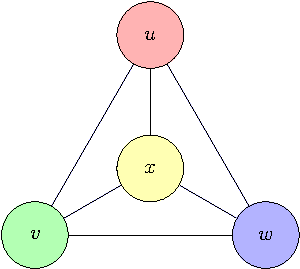
\includegraphics[height=29mm]{Resources/RemoveInternalVertex-Example-1.pdf}}
	\quad
	\subfigure[]{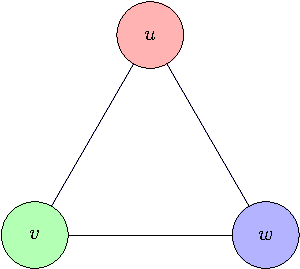
\includegraphics[height=29mm]{Resources/RemoveInternalVertex-Example-2.pdf}}
	\qquad
	\subfigure[]{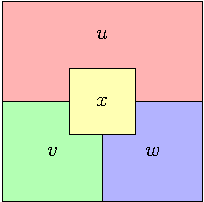
\includegraphics[height=29mm]{Resources/RemoveInternalVertex-Example-3.pdf}}
	\quad
	\subfigure[]{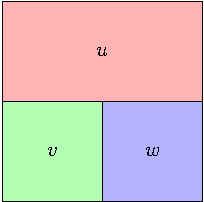
\includegraphics[height=29mm]{Resources/RemoveInternalVertex-Example-4.pdf}}
	\caption{A cluster graph and a polygonal dual thereof, before (a, b) and after (c, d) removing the internal vertex $x$ with degree 3.}
	\label{fig:remove-internal-vertex-example}
\end{figure}

\begin{itemize}
	\item compute boundary (path) with the three incident faces: $u$-$x$, $v$-$x$, $w$-$x$
	\item let one of the incident faces annex the area :D
\end{itemize}

\lipsum



\paragraph{Removing External Vertices}

When removing vertices on the outer face along with its incident edges, we must ensure that the graph remains 2-connected afterwards. \cref{fig:remove-external-vertex-example} illustrates a valid removal of a vertex on the outer face.

\begin{figure}[H]
	\centering
	\subfigure[]{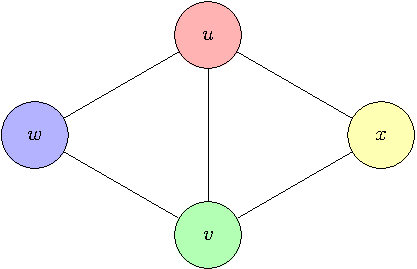
\includegraphics[height=29mm]{Resources/RemoveExternalVertex-Example-1.pdf}}
	\quad
	\subfigure[]{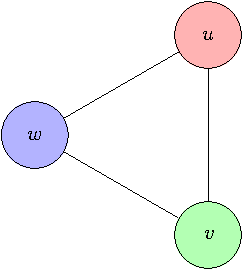
\includegraphics[height=29mm]{Resources/RemoveExternalVertex-Example-2.pdf}}
	\qquad
	\subfigure[]{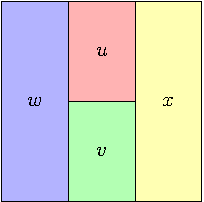
\includegraphics[height=29mm]{Resources/RemoveExternalVertex-Example-3.pdf}}
	\quad
	\subfigure[]{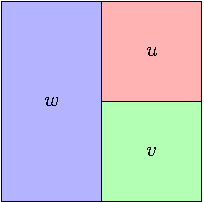
\includegraphics[height=29mm]{Resources/RemoveExternalVertex-Example-4.pdf}}
	\caption{A cluster graph and a polygonal dual thereof, before (a, b) and after (c, d) removing the vertex $x$ on the outer face.}
	\label{fig:remove-external-vertex-example}
\end{figure}

\begin{itemize}
	\item find boundary of respective face with outer face
	\item remove all internal/subdivision vertices and edges on this path
\end{itemize}

\lipsum
